\section{Ejercicio 2: Reconocimiento de secuencia de bits}
Se desea dise\~nar una m\'aquina de estados implementada con m\'aquina de Mealy, la cual sea capaz de analizar una secuencia de bits y detectar si se produjo un patr\'on
seguido por 1-1-0-1, ante lo cual deber\'a notificar tal suceso activando su salida para ello. En la Fig. \ref{fig:esquema_general_dispositivo} se ilustra un esquema general de ello.

\begin{figure}[H]
    \centering
    \includegraphics[scale=0.7]{../EJ2/Recursos/dispositivo_general.png}
    \caption{Esquema general del dispositivo a dise\~nar}
    \label{fig:esquema_general_dispositivo}
\end{figure}

\subsection{Dise\~no de M\'aquina de Estados}
En primer lugar, dadas las especificaciones de la m\'aquina de estado, se desea dise\~nar tal dispositivo el cual consta de una \'unica entrada y una \'unica salida. Para lo cual se
emplea un esquema gen\'erico de m\'aquina de estados, en donde la salida ser\'a asincr\'onica pues se busca utilizar el dise\~no de Mealy para tal l\'ogica. Este esquema general descripto
puede visualizarse en la Fig. \ref{fig:esquema_general_mealy}, donde la cantidad de entradas no es necesariamente la misma que en la salida.

\begin{figure}[H]
    \centering
    \includegraphics[scale=0.7]{../EJ2/Recursos/maquina_estados_mealy.png}
    \caption{Esquema general de la m\'aquina de Mealy}
    \label{fig:esquema_general_mealy}
\end{figure}

En la Fig. \ref{fig:diagrama_estados_ejercicio_2} se puede observar el diagrama de estados propuesto. Es importante mencionar que el estado de Reset es definido como tal
para reconocer cu\'al es el estado inicial de la m\'aquina, y deber\'a ser tenido en cuenta durante la asignaci\'on de estados en caso de proveer la posibilidad de reiniciar la m\'aquina,
pues los flip flops deber\'an ser llevados a dicho estado, seg\'un sea asignado.

\begin{figure}[H]
    \centering
    \includegraphics[scale=0.6]{../EJ2/Recursos/diagrama_estados.png}
    \caption{Diagrama de estados}
    \label{fig:diagrama_estados_ejercicio_2}
\end{figure}

En la Tabla \ref{table:tabla_estados_ejercicio_2} se puede observar la tabla de estados o transiciones de la m\'aquina de estados, habiendo ya asignado correspondientemente a cada estado una configuraci\'on de bits. Es de inter\'es mencionar
que tal asignaci\'on es el resultado de comparar las diferentes alternativas y encontrar que, dada la distribuci\'on propuesta, la l\'ogica externa es la m\'inima necesaria.

\begin{table}[H]
    \centering
    \begin{tabular}{c  c c  c c}
        Estado & \multicolumn{2}{c}{Pr\'oximo} & \multicolumn{2}{c}{Salida} \\
        $y_2 y_1$ & $w = 0$ & $w = 1$ & $w = 0$ & $w = 1$ \\
        \hline \\
        $A=11$ & $A=11$ & $B=00$ & $z=0$ & $z=0$ \\
        $B=00$ & $A=11$ & $C=01$ & $z=0$ & $z=0$ \\
        $C=01$ & $D=10$ & $C=01$ & $z=0$ & $z=0$ \\
        $D=10$ & $A=11$ & $A=11$ & $z=0$ & $z=1$ \\
        \hline
    \end{tabular}    
    \caption{Tabla de estados o transiciones}
    \label{table:tabla_estados_ejercicio_2}
\end{table}

\begin{figure}[H]
    \centering
    \begin{Karnaughvuit}
    \maxterms{0,1,2,3,4,5,7}
    \minterms{6}
    \implicantsol{6}{red}
    \end{Karnaughvuit}
    \caption{Karnaugh para la variable de salida}
\end{figure}

\begin{equation}
    z = w \cdot y_2 \cdot \overline{y_1}
\end{equation}

\begin{figure}[H]
    \centering
    \begin{Karnaughvuit}
    \maxterms{4,5,7}
    \minterms{0,1,2,3,6}
    \implicant{0}{2}{red}
    \implicant{2}{6}{blue}
    \end{Karnaughvuit}
    \caption{Karnaugh para la variable de estado $y_2$}
\end{figure}

\begin{equation}
    y_2 = \overline{w} + y_2 \cdot \overline{y_1}
\end{equation}

\begin{figure}[H]
    \centering
    \begin{Karnaughvuit}
    \maxterms{1,7}
    \minterms{0,2,3,4,5,6}
    \implicant{4}{5}{red}
    \implicant{3}{2}{red}
    \implicantcostats{0}{6}{blue}
    \end{Karnaughvuit}
    \caption{Karnaugh para la variable de estado $y_1$}
\end{figure}

\begin{equation}
    y_1 = \overline{y_1} + \overline{w} \cdot y_2 + w \cdot \overline{y_2}
\end{equation}

\subsection{Simulaciones en Verilog}
En la Fig. \ref{fig:circuito_logico_ej2} se puede observar el circuito l\'ogico completo correspondiente a la m\'aquina de estados dise\~nada
en el apartado anterior. Se desea comprobar su correcto funcionamiento a nivel l\'ogico mediante una simulaci\'on en Verilog, para lo cual se emplean
dos metodolog\'ias de dise\~no.

Por un lado, puede utilizarse un dise\~no en Verilog que determine si la m\'aquina est\'a bien diagramada, utilizando para ello el bloque producedural case.
Por otro lado, para determinar si la implementaci\'on l\'ogica de la m\'aquina puede funcionar, debe emplearse un dise\~no a nivel compuertas de los m\'odulos en Verilog,
para esto \'ultimo se divide el problema inicialmente en tres bloques, los flip flops, la l\'ogica combinacional que produce el pr\'oximo estado y la l\'ogica de salida. Finalmente,
un cuarto bloque o m\'odulo describe la m\'aquina interconectando los m\'odulos mencionados para producir el comportamiento esperado.

\begin{figure}[H]
    \centering
    \includegraphics[scale=0.5]{../EJ2/Recursos/circuito_logico.png}
    \caption{Circuito l\'ogico completo de la m\'aquina de estados}
    \label{fig:circuito_logico_ej2}
\end{figure}

En la Fig. \ref{fig:ej2_simulacion} se muestra a modo de referencia la simulaci\'on realizada y visualizada con GTKWave. Para determinar los casos de pruebas de la m\'aquina,
se parti\'o del diagrama de estados y se consideraron diferentes secuencias. En primer lugar la secuencia 0-1-0 para determinar si permanece correctamente en el primer estado,
pasa al segundo y vuelve al detectar el error. En segundo lugar, la secuencia 1-1-1-0-0, para determinar si llega correctamente al tercer estado, permanece y luego transiciona reiniciando
la m\'aquina pero con la salida en estado bajo. Finalmente, la secuencia correcta para analizar si la salida responde como es esperado.

\begin{figure}[H]
    \centering
    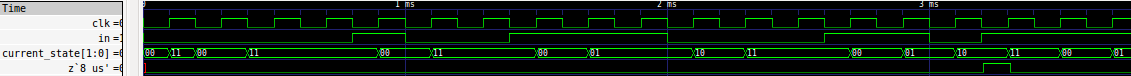
\includegraphics[scale=0.4]{../EJ2/Recursos/simulacion.png}    
    \caption{Simulaci\'on de Verilog visualizada con GTKWave}
    \label{fig:ej2_simulacion}
\end{figure}

\subsection{Dise\~no en PCB}
La realizaci\'on del PCB para implementar el circuito l\'ogico implica la conexi\'on de las compuertas l\'ogicas siguiendo
el esquema te\'orico, y verificando previamente que no hayan complicaciones f\'isicas en tales conexiones. Esto \'ultimo implica
utilizar consistentemente tecnolog\'ia TTL, verificando que las corrientes de salida de las compuertas no sea superada con el consumo
de las entradas, es decir no superar el fan-out. Adem\'as, para prevenir fallos por picos en la tensi\'on de alimentaci\'on durante transitorios de las compuertas,
se conectaron los debidos capacitores de desacople.

\begin{figure}[H]
    \centering
    \begin{tabular}{c c}
        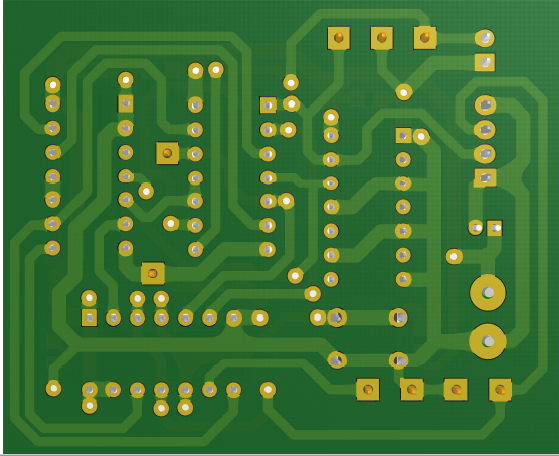
\includegraphics[scale=0.45]{../EJ2/Recursos/pcb_3d_bottom.PNG} & 
        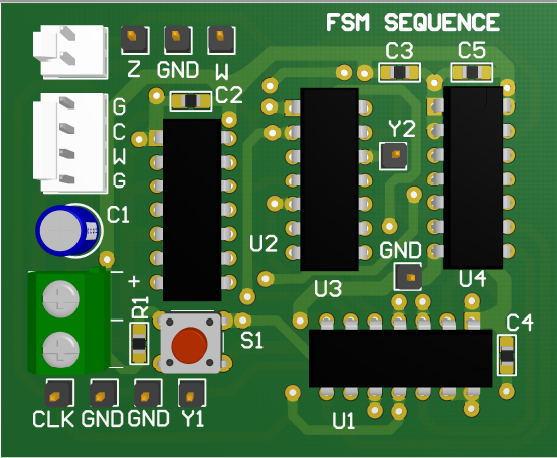
\includegraphics[scale=0.45]{../EJ2/Recursos/pcb_3d_top.PNG} \\
        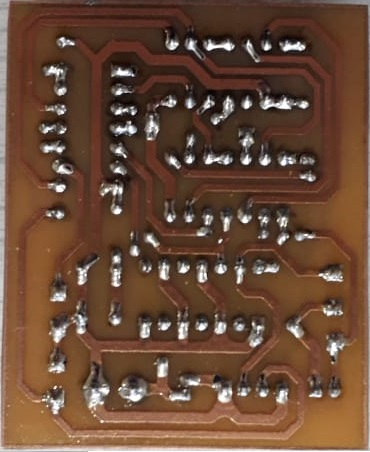
\includegraphics[scale=0.6]{../EJ2/Recursos/pcb_bottom.jpeg} & 
        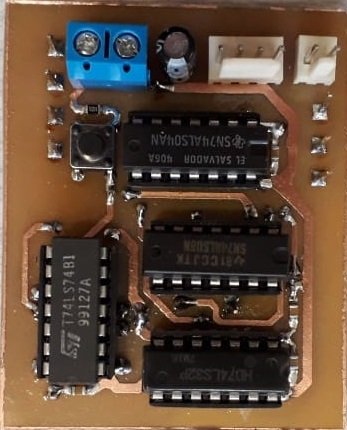
\includegraphics[scale=0.6]{../EJ2/Recursos/pcb_top.jpeg} \\
    \end{tabular}
    \caption{PCB dise\~nado e implementado}
\end{figure}

\subsection{Resultados}
Para la verificaci\'on del correcto funcionamiento se propone poner bajo prueba al circuito con las mismas tres secuencias que fueron empleadas
en el proceso de simulaci\'on. Estas secuencias son 0-1-0, 1-1-1-0-0 y 1-1-0-1, para lo cual se utiliza una se\~nal de clock de baja frecuencia y la
entrada se controla con un pulsador externo al PCB, y se realizan estas mediciones en dos partes para poder extraer la informaci\'on de la salida y la de los estados,
ya que s\'olo se dispone de osciloscopio de cuatro canales.

En la Fig. \ref{fig:fsm_ejercicio_2_estados} se muestran las mediciones de los estados de la m\'aquina de estados, en donde las se\~nales Amarilla, Verde, Azul y Roja/Rosa,
corresponden respectivamente a la se\~nal de clock, la entrada $w$, el bit de estado $y_2$ y el bit de estado $y_1$. Mientras que en la Fig. \ref{fig:fsm_ejercicio_2_salida} se mide
la salida de la m\'aquina de estados, en donde la se\~nales Amarilla, Verde y Azul, corresponden respectivamente a la se\~nal de clock, la entrada $w$ y la salida $z$.

De izquierda a derecha, de arriba hacia abajo se ordenan los casos de cada secuencia seg\'un fueron mencionados anteriomente.

\begin{figure}[H]
    \centering
    \begin{tabular}{c c}
        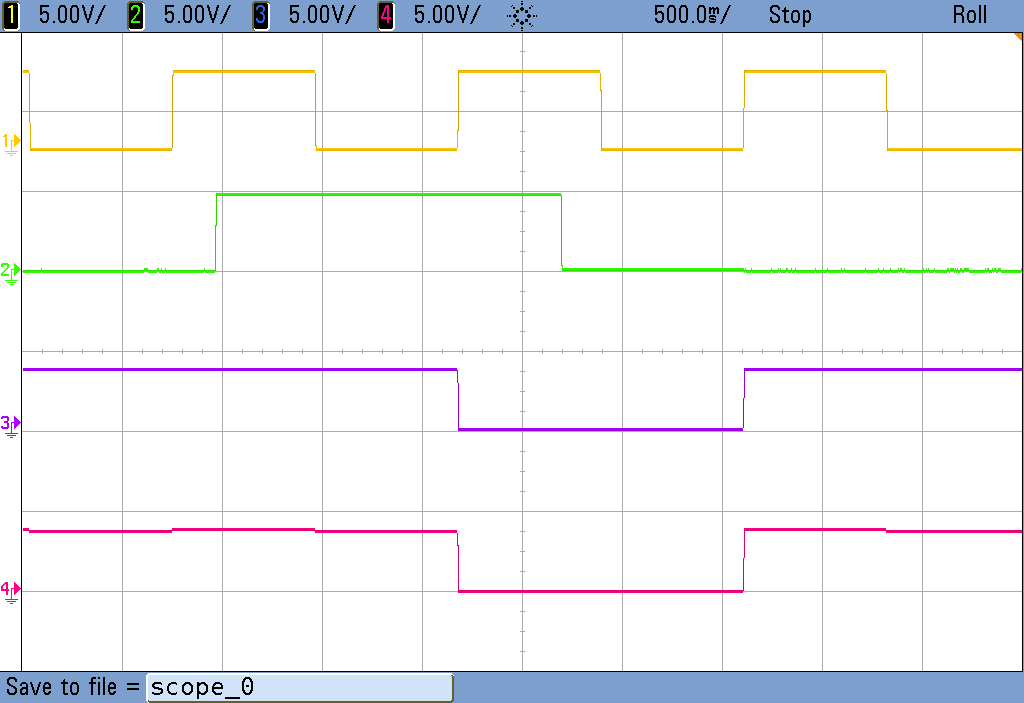
\includegraphics[scale=0.2]{../EJ2/Mediciones/Estados/cropped_scope_0.png} & 
        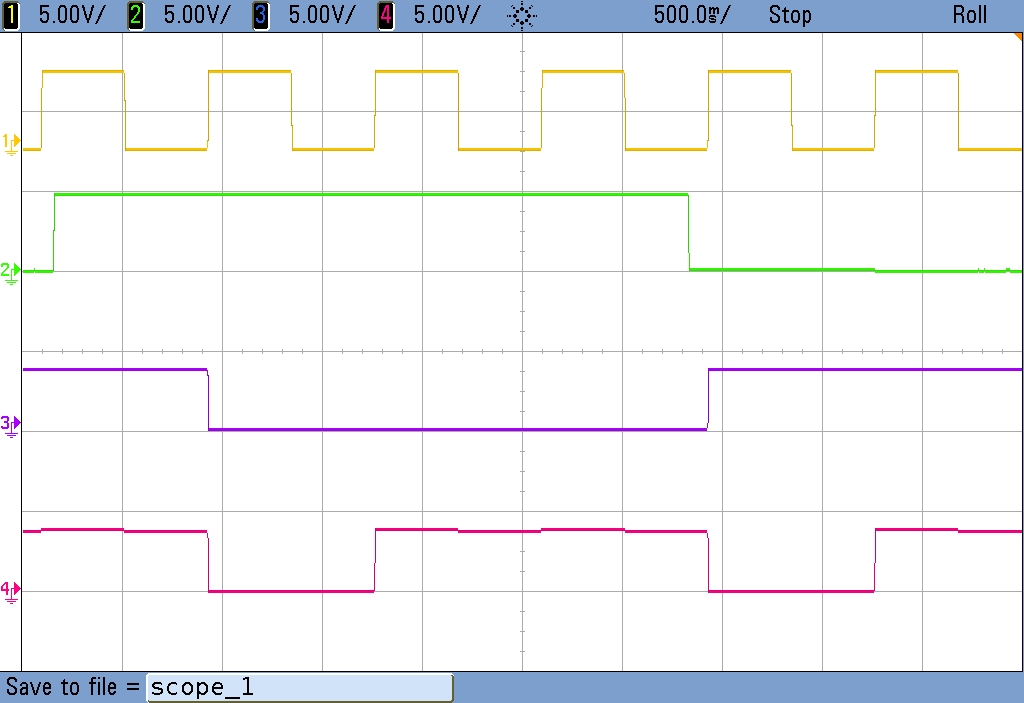
\includegraphics[scale=0.2]{../EJ2/Mediciones/Estados/cropped_scope_1.png} \\ 
    \end{tabular}
    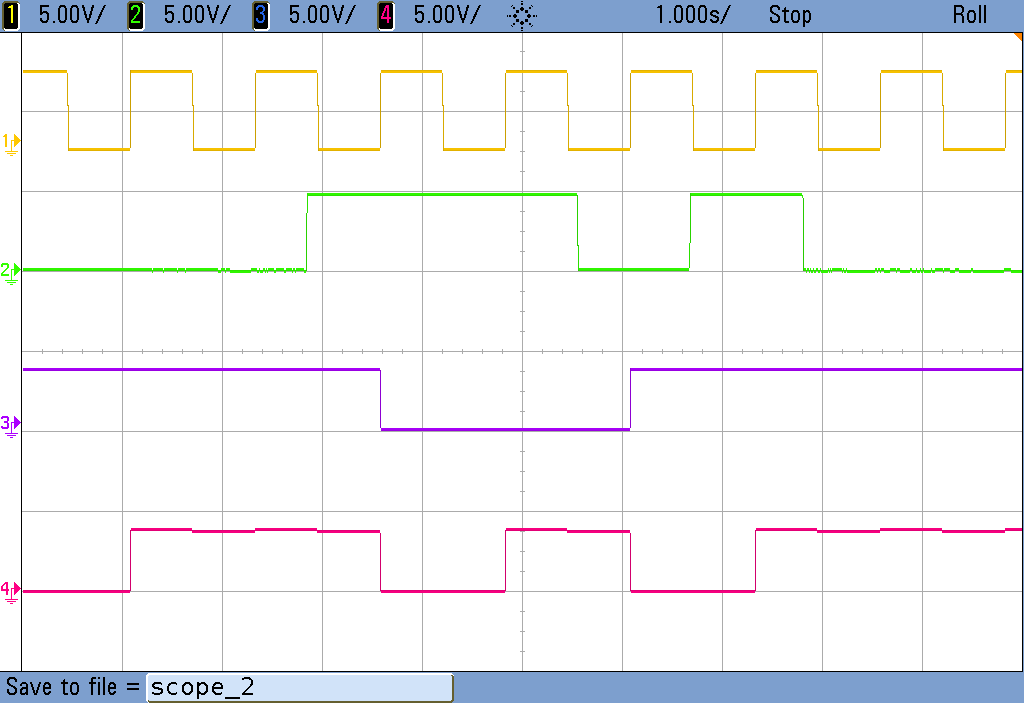
\includegraphics[scale=0.2]{../EJ2/Mediciones/Estados/cropped_scope_2.png}
    \caption{Estados de la FSM}
    \label{fig:fsm_ejercicio_2_estados}
\end{figure}

\begin{figure}[H]
    \centering
    \begin{tabular}{c c}
        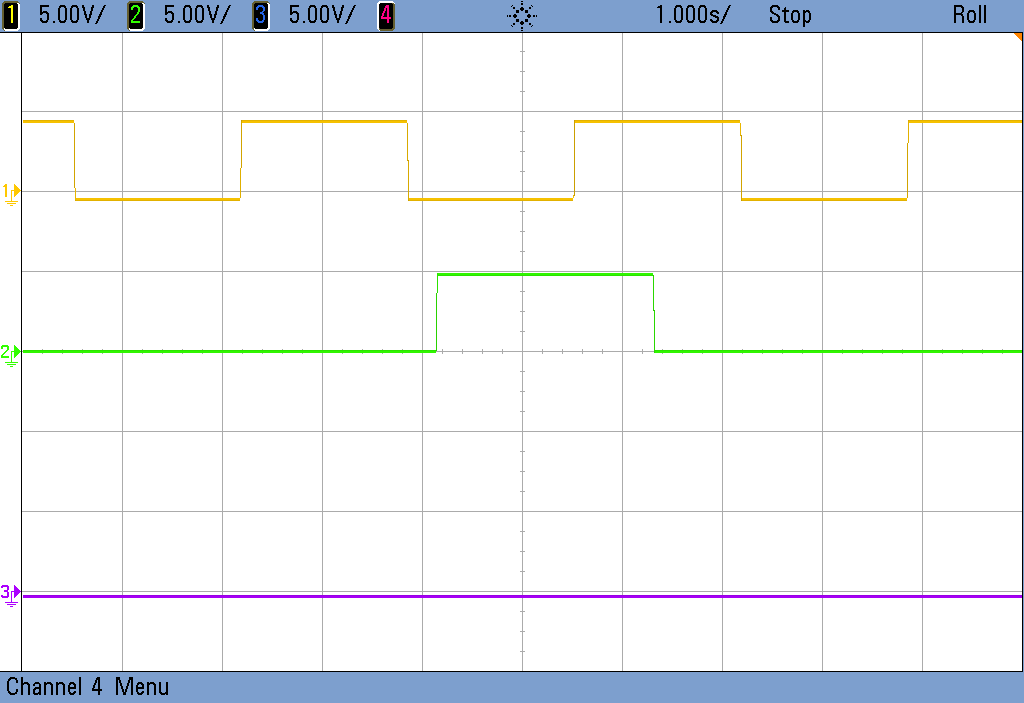
\includegraphics[scale=0.2]{../EJ2/Mediciones/Salida/cropped_scope_3.png} & 
        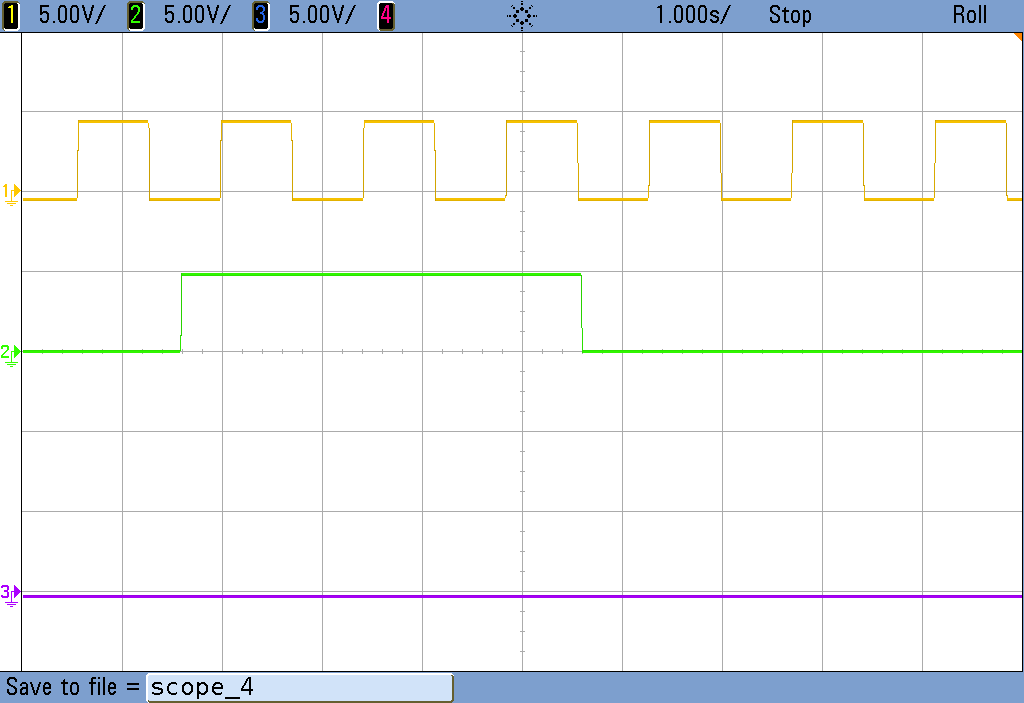
\includegraphics[scale=0.2]{../EJ2/Mediciones/Salida/cropped_scope_4.png} \\ 
    \end{tabular}
    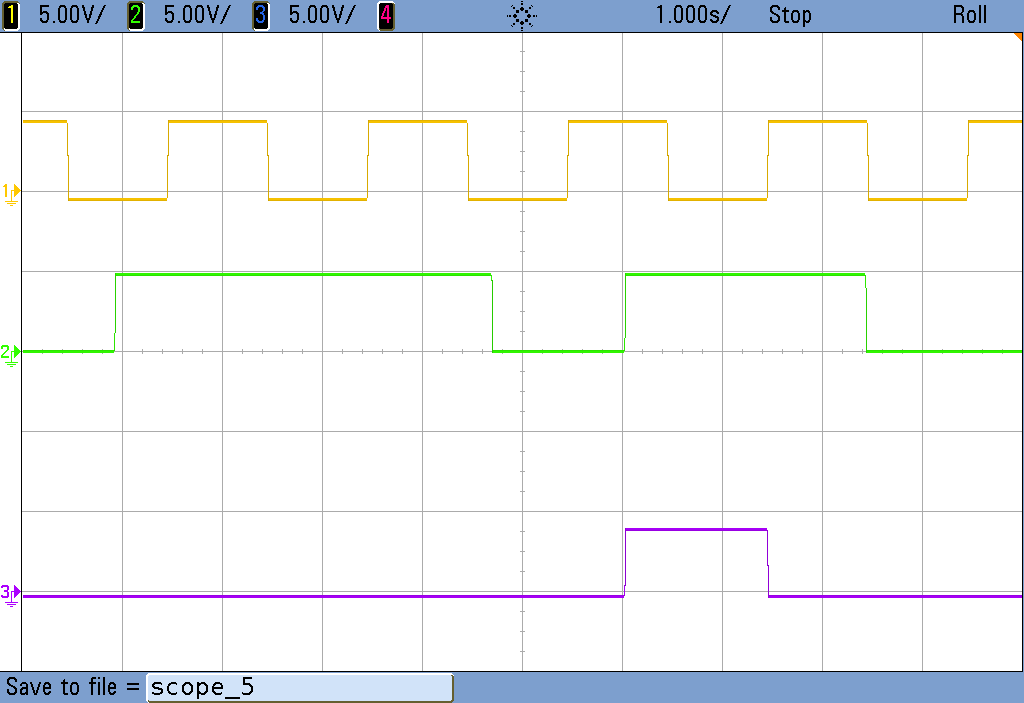
\includegraphics[scale=0.2]{../EJ2/Mediciones/Salida/cropped_scope_5.png}
    \caption{Salida de la FSM}
    \label{fig:fsm_ejercicio_2_salida}
\end{figure}

\subsection{Conclusiones}
Consid\'erese la m\'aquina de estados dise\~nada en base al reconocimiento de una secuencia de 4 bits, luego
para el caso de una m\'aquina de Moore se necesitar\'ia un estado adicional donde luego de detectar la secuencia se mantenga la salida en un estado alto. Por otro lado,
considerando los tiempos de propagaci\'on, para el instante del flanco ascendente en el cual la secuencia correcta es identificada, la salida no necesariamente refleja tal detecci\'on
sino hasta pasar un determinado tiempo, como consecuencia de su sincronismo.
Estos aspectos evidencian por qu\'e una m\'aquina de Mealy puede resultar beneficiosa, dado que hace uso de menos estados, y su salida al ser asincr\'onica permite que
para el flanco de detecci\'on de la secuencia la salida refleje haber detectado correctamente el patr\'on.
